%\textit{In this section, I will present and analyse 4 different approached to improve the stability of optimal portfolios. I will keep the description of the first 3 methods short. However, I don't want to remove them completely because I would like to compare the results of those 3 "simpler" methods to the "more complex" Hierarchical Risk Parity method.}

In this section, we present two methods that try to improve the stability of Markowitz's minimum volatility portfolios. The first method, called covariance matrix shrinking, tries to tackle instability by reducing noise in the sample covariance matrix: if the input covariance matrix does not change dramatically across time, then the resulting optimal portfolio won't change dramatically across time either. The second method, called hierarchical risk parity, is an intermediate optimisation method between Markowitz's minimum variance portfolio and the inverse variance portfolio and was developed by López de Prado: instead of considering stochastic dependency between the returns of different assets via their covariances directly, assets are classified in clusters according to their correlation first, and then wealth is allocated across the mentioned clusters so that they contribute to the total portfolio risk in equal proportions.

\subsection{Covariance Matrix Shrinking}
    %\textit{This method tries to improve stability by reducing noise in the sample covariance matrix. It is easy to implement and I believe it is also to interpret by analysing the condition number of the shrunk covariance matrix.}
	
	In Markowitz's minimum volatility portfolio construction method, the only input variable that we have is the covariance matrix of asset returns. Hence, the covariance matrix is the only source of instability and errors in the process of portfolio optimisation for this method. We have already shown this in our practical implementation in section \ref{section:MarkowitzsCurse}.
	
	In section \ref{section:MarkowitzPracticalImplementation}, we have used the sample covariance matrix computed using NumPy's \texttt{.cov()} method applied to the matrix containing the time-series of past returns of each of the $N$ investable assets. This method computes the unbiased sample covariance matrix of the past returns' time-series. Hence, the most important parameter for the covariance matrix estimation is the number of past periods returns in our time-series.
	
	As we have already described in theorem \ref{theorem:CovarianceMatrixRank}, we need at least as many past returns' observations as investable assets, so that our covariance matrix can be invertible (even though this does not guarantee invertibility). This is not a problem in our practical implementation, because we consider a relatively small set of investable assets. Nevertheless, one can think of asset managers constructing portfolios using a way bigger set of investable assets, for example equal to the S\&P500 index, that contains almost 500 companies. For them, having enough past returns' observations is not necessarily a simple condition to fulfil for all investable assets. Moreover, we have also shortly discussed the trade-off between long and short look-back periods, i.e. for high and low number of past returns' observations $T$. Table \ref{tab:tvaluetradeoff} summarises the advantages and disadvantages of choosing a low and a high number of past returns' observations to estimate the covariance matrix of asset returns irrespective of the value of $N$.
	
%	\begin{table}[h!]
%	    \centering
%	    \begin{tabular}{c|cc}
%	         & Low $T$ & High $T$ \\
%	         \hline
%	         Advantages & React to market changes quicker/sooner. & More stable optimal portfolio across time, i.e. lower turnover. \\
%	         Disadvantages & blabla & blabla
%	    \end{tabular}
%	    \caption{$T$ Value Trade-off}
%	    \label{tab:tvaluetradeoff}
%	\end{table}
	

    \begin{table}[h!]
        \centering
        \begin{tabularx}{\textwidth}{c|XX}
             & \textbf{Low $T$} & \textbf{High $T$} \\
	         \hline
            Advantages & React to market changes quicker/sooner. & More stable portfolios, lower turnover. \\
            Disadvantages & Less stable portfolios, higher turnover & React to market changes slower/later.
        \end{tabularx}
        \caption{$T$ Value Trade-off}
	    \label{tab:tvaluetradeoff}
    \end{table} 
	
	On the one hand, we can choose a low number of past returns' observations to construct our covariance matrix. Doing this will result in covariance matrices that are more volatile, i.e. do change a lot across time. The estimation will be more sensitive to changes in market regimes and changes in asset returns' relationships, but also to noise, which will lead to more unstable portfolios and to higher portfolio turnover across time. On the other hand, we can also choose a high number of past returns' observations to construct our covariance matrix. This will help to get covariance matrices that are more stable across time, producing optimal portfolios that are also more stable across time and hence reducing turnover. However, this portfolios will also be more inelastic to changes in market regimes and changes in asset returns' relationships. As a practical example, one can think about the changes in performance across the different equity sectors during a business cycle: some sectors like financials tend to perform better during periods of high inflation, while other sectors like IT tend to perform worse \cite{fidelitybusinesscycles}. Investors would like to get optimal portfolios that react to those changes in business cycles in order to profit from the out-performance of some asset classes and sectors, while protecting their portfolios from the under-performance of some other asset classes and sector. Moreover, optimal portfolios constructed on the noise abundant in financial time-series should be avoided, so as to reduce turnover.
	
	Optimising this trade-off is the objective of the covariance matrix shrinkage methods.
	
	\subsubsection{Ledoit and Wolf}\label{ledoitwolfsubsection}\todo[inline]{Revisit paper to add further notes that I might have forgotten}
	    Ledoit and Wolf propose using a convex combination of the sample covariance matrix and a structured estimator, i.e. some matrix containing little noise and which is estimated with high bias. The idea is to reduce the noise contained in the sample covariance matrix by compensating positive and negative error that tends to be contained in its highest entries in absolute value. These high absolute-valued entries of the covariance matrix tend to be high absolute-value mostly because of noise and not because the covariance of the corresponding asset returns' time-series is truly high \cite{michaudreturnsstability}.
    	
    	\begin{definition}[Shrunk Covariance Matrix \cite{ledoit}]\label{shrunkcovariancematrixdefinition}
    	    Let $\Sigma \in \mathbb{R}^{N \times N}$ be a sample covariance matrix and $F \in \mathbb{R}^{N \times N}$ some other matrix, also called \textbf{shrinkage target}. The \textbf{shrunk covariance matrix} is given by
    	    \begin{align*}
    	        \Sigma_{shrunk} := \delta F + (1-\delta) \Sigma
    	    \end{align*}
    	    where $\delta \in [0, 1 ]$ is called \textbf{shrinkage constant}.
    	\end{definition}
    	
    	In definition \ref{shrunkcovariancematrixdefinition}, we have 2 parameters apart from the sample covariance matrix $\Sigma$ that we need to further specify: the shrinkage target and the shrinkage constant.
    	
    	For the first, the shrinkage target, we need some estimator that can be computed using few parameters, i.e. a structured estimator, and that also contains important information about the measure that we are trying to estimate, i.e. the stochastic dependency between the random variables of the asset returns. In \cite{ledoit2003}, the authors propose using the single-factor matrix of Sharpe as the shrinkage target, which is a single-index asset pricing model \cite{sharpesim}. However, in \cite{ledoit}, the same authors propose a simpler estimator as shrinkage target.
    	
    	\begin{definition}[Constant Correlation Model \cite{ledoit}]
    	    Let $\Sigma := [\sigma_{i,j}]_{i,j= \{1, \dots, N \}} \in \mathbb{R}^{N \times N}$ be the sample covariance matrix, then the \textbf{sample constant correlation matrix $F_{\Sigma}$ corresponding to the sample covariance matrix $\Sigma$} is defined as
    	    \begin{align*}
    	        F_{\Sigma} := [f_{i,j}]_{i,j= \{1, \dots, N \}} \in \mathbb{R}^{N \times N}, \quad \textbf{where} \quad f_{i,j} := \begin{cases}
    	        \sigma_{i,i} &\quad \text{for } i=j \\
    	        \bar{r} \sqrt{\sigma_{i,i} \sigma_{j,j}} &\quad \text{for } i \neq j
    	        \end{cases}
    	    \end{align*}
    	    and $\bar{r} \in \mathbb{R}$ is the average sample correlation, which can be expressed as
    	    \begin{align}\label{averagesamplecorrelation}
                \bar{r} := \frac{2}{(N-1) N} \sum_{i=1}^{N-1} \sum_{j=i+1}^N \frac{\sigma_{i,j}}{\sqrt{\sigma_{i,i} \sigma_{j,j}}}
    	    \end{align}
    	\end{definition}
    	
    	Ledoit and Wolf argue that the constant correlation model gives comparable performance while being easier to implement than the single-factor matrix model of Sharpe \cite{ledoit}. However, they also mention that the constant correlation model is suited for portfolio construction if the set of investable assets contains assets from different classes, for example fixed-income and equities, because it assumes that all pairwise correlations are treated equal for the computation of the average sample correlation $r$. From an economic perspective, this makes sense because the returns of different asset classes can be driven by very different factors: for example, while the stock returns of technology companies are often driven by their margins and customer base growth, the bond returns of the same companies are rather driven by the liquidity of their balance sheet. Nevertheless, we consider this shrinkage target in our practical implementation, because our backtesting period is marked by the market-stress caused by the COVID-19 crisis, and the asset returns during this kind of periods tend to be driven by macroeconomic factors across the different asset classes.
    	
    	The second parameter in definition \ref{shrunkcovariancematrixdefinition}, the shrinkage constant, represents the compromise between the sample covariance matrix and the structured estimator. It can take infinite many different values, even if constrained to be in the interval $[0,1]$ so as to compute the shrunk covariance matrix as a convex combination of the structured estimator and the sample covariance matrix. Ledoit and Wolf propose defining the shrinkage constant as the optimal $\delta^* \in [0,1]$ that minimises the distance between the shrunk covariance matrix and the true covariance matrix, i.e. the covariance matrix that contains the covariances of investable asset returns without noise.
    	
    	\begin{theorem}[\cite{ledoit2003}]\label{optimalshrinkageconstantheorem}
    	        Let $S := [s_{i,j}]_{i,j= \{1, \dots, N \}} \in \mathbb{R}^{N \times N}$ be the sample covariance matrix computed using $T \in \mathbb{N}$ past returns observations, $F_S := [f_{i,j}]_{i,j= \{1, \dots, N \}} \in \mathbb{R}^{N \times N}$ the sample constant correlation matrix corresponding to $S$, $\Sigma := [\sigma_{i,j}]_{i,j= \{1, \dots, N \}} \in \mathbb{R}^{N \times N}$ the true covariance matrix and $F_\Sigma := [\phi_{i,j}]_{i,j= \{1, \dots, N \}} \in \mathbb{R}^{N \times N}$ its constant correlation matrix. Moreover, we define the loss function
    	        \begin{align*}
    	            L(\delta) = \| \delta F_S + (1-\delta) S - \Sigma \|_F
    	        \end{align*}
    	        where $\| \cdot \|_F$ is the Frobenius norm. The shrinkage constant $\delta^*$ that minimises the expected value of $L$ is given by
    	        \begin{align}\label{optimalshrinkageconstant}
    	            \delta^* := \frac{\sum_{i=1}^N \sum_{j=1}^N \mathbb{V}[s_{i,j}] - Cov[f_{i,j}, s_{i,j}]}{\sum_{i=1}^N \sum_{j=1}^N \mathbb{V}[f_{i,j} - s_{i,j}] + (\phi_{i,j} - \sigma_{i,j})^2}
    	        \end{align}
    	        where the function $\mathbb{V}[\cdot]$ designates the variance and $Cov[\cdot, \cdot]$ the covariance.
    	\end{theorem}
    	
    	The proof of this theorem is provided in \cite{ledoit2003} and goes as follows.
    	
    	\begin{proof}
    	        The expected value of the loss function $L$ can be rewritten as
    	        \begin{align*}
    	            \mathbb{E}[L(\delta)] &= \sum_{i=1}^N \sum_{j=1}^N \mathbb{E}[\delta f_{i,j} + (1- \delta) s_{i,j} - \sigma_{i.j}]^2 \\
    	            &= \sum_{i=1}^N \sum_{j=1}^N \mathbb{V}[\delta f_{i,j} + (1 - \delta) s_{i,j}] + (\mathbb{E}[\delta f_{i,j} + (1- \delta) s_{i,j} - \sigma_{i,j}])^2 \\
    	            &= \sum_{i=1}^N \sum_{j=1}^N \delta^2 \mathbb{V}[f_{i,j}] + (1 - \delta)^2 \mathbb{V}[s_{i,j}] + 2 \delta (1 - \delta) Cov[f_{i,j}, s_{i,j}] + \delta^2 (\phi_{i,j} - \sigma_{i,j})^2
    	        \end{align*}
    	        The first and second derivatives of the expected value of the loss function $L$ with respect to $\delta$ are given by
    	        \begin{align*}
    	            \frac{\partial L}{\partial \delta} &= 2 \sum_{i=1}^N \sum_{j=1}^N \delta \mathbb{V}[f_{i,j}] - (1 - \delta) \mathbb{V}[s_{i,j}] + (1- 2 \delta) Cov[f_{i,j}, s_{i,j}] + \delta (\phi_{i,j} - \sigma_{i,j})^2 \\
    	            \frac{\partial^2 L}{\partial \delta^2} &= 2 \sum_{i=1}^N \sum_{j=1}^N \mathbb{V}[f_{i,j} - s_{i,j}] + (\phi_{i,j} - \sigma_{i,j})^2
    	        \end{align*}
    	        Because $ \frac{\partial^2 L}{\partial \delta^2} > 0$ holds, the minimum of the expected value of the loss function $L$ can be computed by setting $\frac{\partial L}{\partial \delta}$ equal to zero. Solving for $\delta^*$ we get
    	        \begin{align*}
    	            \delta^* = \frac{\sum_{i=1}^N \sum_{j=1}^N \mathbb{V}[s_{i,j}] - Cov[f_{i,j}, s_{i,j}]}{\sum_{i=1}^N \sum_{j=1}^N \mathbb{V}[f_{i,j} - s_{i,j}] + (\phi_{i,j} - \sigma_{i,j})^2}
    	        \end{align*}
    	\end{proof}
    	
    	The only problem of the optimal shrinkage constant presented in theorem \ref{optimalshrinkageconstantheorem} is that we don't know the true covariance matrix and can only compute sample variances and covariances. Therefore, Ledoit and Wolf propose using a consistent estimator for $\delta^*$, i.e. an estimator that converges to the true $\delta^*$ for $T \rightarrow \infty$.
    	
    	\begin{theorem}[\cite{ledoit}]
    	    Assuming that asset returns' random variables are independent and identically distributed with finite fourth moment, let $Y := [y_{i,j}]_{i= \{1, \dots, N \}, j= \{1, \dots, T \}} \in \mathbb{R}^{N \times T}$, where $y_{i,j}$ represents the return of the ith asset in the past jth period, and $\bar{y}_i := \sum_{j=1}^T y_{i,j}$. Moreover, we define the matrices $S := [s_{i,j}]_{i,j= \{1, \dots, N \}} \in \mathbb{R}^{N \times N}$ as the sample covariance matrix computed using the returns observations in $Y$, $F_S := [f_{i,j}]_{i,j= \{1, \dots, N \}} \in \mathbb{R}^{N \times N}$ as its sample constant correlation matrix, $\Sigma := [\sigma_{i,j}]_{i,j= \{1, \dots, N \}} \in \mathbb{R}^{N \times N}$ as the true covariance matrix and $F_\Sigma := [\phi_{i,j}]_{i,j= \{1, \dots, N \}} \in \mathbb{R}^{N \times N}$ as its constant correlation matrix. Then
    	    \begin{align*}
    	        \hat{\pi} := \sum_{i=1}^N \sum_{j=1}^N \hat{\pi}_{i,j} \quad \text{where} \quad \hat{\pi}_{i,j} := \frac{1}{T} \sum_{t=1}^T \left( (y_{i,t} - \bar{y}_{i}) (y_{j,t} - \bar{y}_{j}) \right)^2
    	    \end{align*}
    	    is a consistent estimator for $\sum_{i=1}^N \sum_{j=1}^N \mathbb{V}[\sqrt(T) s_{i,j}]$,
    	    \begin{align*}
    	        \hat{\rho} &:= \sum_{i=1}^N \hat{\pi}_{i,i} + \sum_{i=1}^N \sum_{j=1, \; j \neq i}^N \frac{\bar{r}}{2} \left( \sqrt{\frac{s_{j,j}}{s_{i,i}}} \hat{\vartheta}_{i,i,j} + \sqrt{\frac{s_{i,i}}{s_{j,j}}} \hat{\vartheta}_{j,i,j} \right) \\
    	        \text{where} \quad \hat{\vartheta}_{k,i,j} &:= \frac{1}{T} \sum_{t=1}^T \left( (y_{k,t} - \bar{y}_k)^2 - s_{k,k} \right) \left( (y_{i,t} - \bar{y}_i) (y_{j,t} - \bar{y}_j) - s_{i,j} \right)
    	    \end{align*}
    	    and $\bar{r}$ is defined as in equation \ref{averagesamplecorrelation} is a consistent estimator for $\sum_{i=1}^N \sum_{j=1}^N Cov[\sqrt{T} f_{i,j}, \sqrt{T}, s_{i,j}]$ and
    	    \begin{align*}
    	        \hat{\gamma} := \sum_{i=1}^N \sum_{j=1}^N (f_{i,j} - s_{i,j})^2
    	    \end{align*}
    	    is a consistent estimator for $\sum_{i=1}^N \sum_{j=1}^N (\phi_{i,j} - \sigma_{i,j})^2$. Furthermore,
    	    \begin{align*}
    	        \sum_{i=1}^N \sum_{j=1}^N \mathbb{V}[f_{i,j} - s_{i,j}] = O \left( \frac{1}{T} \right)
    	    \end{align*}
    	    Finally, a consistent estimator for the optimal $\delta^*$ defined in equation \ref{optimalshrinkageconstant} is given by
    	    \begin{align}\label{consistentshrinkageconstantestimator}
    	        \hat{\delta}^* := \frac{1}{T} \frac{\hat{\pi} - \hat{\rho}}{\hat{\gamma}}
    	    \end{align}
    	\end{theorem}
    	
    	A proof of this theorem cannot be found in \cite{ledoit} but is given in \cite{ledoit2003}. The assumption of asset returns' random variables being independent and identically distributed with finite moments is necessary to prove convergence using the Central Limit Theorem. Ledoit and Wolf argue that stock returns do not fulfil this assumption, but that covariance matrix estimators also use this assumption and that introducing extra degrees of freedom in the estimation process to account for dependence and conditional heteroskedastic does not necessarily lead to better out-of-sample performance \cite{ledoit2003}.
    	
    	In \cite{ledoit}, Ledoit and Wolf point to the fact that $\hat{\delta}^* \notin [0,1]$ in equation \ref{consistentshrinkageconstantestimator} may hold. Hence, the final shrinkage intensity proposed by Ledoit and Wolf is defined as
    	\begin{align*}
    	    \delta := \max \left\{ 0, \min \left\{ \frac{1}{T} \frac{\hat{\pi} - \hat{\rho}}{\hat{\gamma}}, 1 \right\} \right\}
    	\end{align*}
    	
    	\begin{algorithm}[H]
            \SetAlgoLined
            \SetKwInOut{Input}{Input}\SetKwInOut{Output}{Output}
            \Input{$N$-Asset return matrix $R \in \mathbb{R}^{N \times T}$}
            \Output{Markowitz Minimum Variance Portfolio $w_{opt}$ corresponding to Ledoit and Wolf's shrunk covariance matrix}
            
            Compute the sample covariance matrix $\Sigma \in \mathbb{R}^{N \times N}$\;
            Compute the sample constant correlation matrix $F_{\Sigma} \in \mathbb{R}^{N \times N}$\;
            Compute the shrinkage intensity $\delta := \max \left\{ 0, \min \left\{ \frac{1}{T} \frac{\hat{\pi} - \hat{\rho}}{\hat{\gamma}}, 1 \right\} \right\} \in [0,1]$\;
            Set $\Sigma_{shrunk} := \delta F_{\Sigma} + (1 - \delta) \Sigma$\;
            Set $\Tilde{w}_{opt} \in \mathbb{R}^N$\ as the solution to $\Sigma_{shrunk} \cdot w = \mathds{1}$\;
            Set $w_{opt} = \frac{1}{\mathds{1}^T \cdot \Tilde{w}_{opt}} \cdot \Tilde{w}_{opt}$\;
            \caption{Markowitz Minimum Variance Portfolio Computation with Ledoit and Wolf's Covariance Matrix Shrinkage}
        \end{algorithm}
    
    \subsubsection{De Nard}\todo[inline]{Revisit paper to add further comments that I might have forgotten.}
        In subsection \ref{ledoitwolfsubsection}, we have discussed a covariance matrix shrinkage method that uses the sample constant correlation matrix corresponding to the sample covariance matrix as shrinkage target. As already mentioned before, the disadvantage of this shrinkage target is that all pairwise correlations are weighted equally. However, the pairwise unconditional correlations of assets from different classes (for example of fixed-income vs equity assets) or even of assets from the same class but from different industries or regions are not equal, because the asset returns of different classes are driven by different economic factors.
        
        In \cite{denard}, De Nard proposed a different approach for the covariance shrinkage method, that first clusters the assets in the covariance matrix in homogeneous groups to then shrink the corresponding block matrices inside the covariance matrix by homogeneous group, instead of using the "all-assets-are-equal" approach proposed by Ledoit and Wolf. This approach allows us to apply covariance shrinkage to portfolios composed of assets from different classes (as in our practical implementation) and also account for the different fundamental properties of assets from different industries and regions in the case of portfolios that are homogeneous with respect to asset class.
        
        \begin{definition}[Generalised Constant-Variance-Covariance Shrinkage Target \cite{denard}]\label{gcvcshrinkagetargetdefinition}
            Let $K \in \mathbb{N}$ be the number of homogeneous groups in which we cluster the $N \in \mathbb{N}$ assets, such that $K \leq N$. Without loss of generality, assume that the covariance matrix of asset returns is given by
            \begin{align*}
                \Sigma := \begin{bmatrix}
                    \Sigma_{1,1} & \Sigma_{1,2} & \dots & \Sigma_{1,K} \\
                    \Sigma_{2,1} & \Sigma_{2,2} & \dots & \Sigma_{2,K} \\
                    \vdots & \vdots & \ddots & \vdots \\
                    \Sigma_{K,1} & \Sigma_{K,2} & \dots & \Sigma_{K,K}
                \end{bmatrix} \in \mathbb{R}^{N \times N}
            \end{align*}
            where $\Sigma_{i,j} = \left[ \sigma_{l,m}^{i,j} \right]_{l=1, \dots, N_i; m=1, \dots, N_j} \in \mathbb{R}^{N_i, N_j}$ is the covariance matrix between the assets in the $i$-th and $j$-th homogeneous groups.
            
            We define the \textbf{generalised constant-variance-covariance (GCVC) shrinkage target} as
            \begin{align*}
                \Phi_{GCVC} := \begin{bmatrix}
                \Phi_{1,1} & \Phi_{1,2} & \dots & \Phi_{1,K} \\
                \Phi_{2,1} & \Phi_{2,2} & \dots & \Phi_{2,K} \\
                \vdots & \vdots & \ddots & \vdots \\
                \Phi_{K,1} & \Phi_{K,2} & \dots & \Phi_{K,K}
                \end{bmatrix} \in \mathbb{R}^{N \times N}
            \end{align*}
            where $\Phi_{i,j} \in \mathbb{R}^{N_i, N_j}$ is the $(i,j)$-th cluster of $\Phi_{GCVC}$ and is defined as
            \begin{align*}
                \Phi_{i,j} := \begin{cases}
                \varphi_k I_{N_k} + \nu_k \left( \mathds{1}_{N_k} \mathds{1}_{N_k}^T - I_{N_k} \right) \quad &\text{for } i = j = k \in \{ 1, \dots, K \} \\
                \nu_{i,j} \mathds{1}_{N_i} \mathds{1}_{N_j}^T \quad &\text{for } i \neq j \in \{ 1, \dots, K \}
                \end{cases}
            \end{align*}
            where $N_k$ is the number of assets in group $k$, $I_{N_k}$ is the $N_k$-dimensional identity matrix and $\mathds{1}_{N_k}$ is the $N_k$-dimensional vector of ones for all $k \in \{ 1, \dots, K \}$. Moreover, $\varphi_k, \nu_k, \nu_{i,j}$ are the average variance of group $k$, the average covariance of group $k$ and the average covariance of the off-diagonal cluster $i,j$ respectively, i.e.
            \begin{align*}
                \varphi_k &:= \frac{1}{N_k} \sum_{l=1}^{N_k} \sigma_{l,l}^{k,k} \\
                \nu_k &:= \frac{1}{N_k^2} \sum_{l=1}^{N_k} \sum_{m=1}^{N_k} \sigma_{l,m}^{k,k} \\
                \nu_{i,j} &:= \frac{1}{N_i N_j} \sum_{l=1}^{N_i} \sum_{m=1}^{N_j} \sigma_{l,m}^{i,j}
            \end{align*}
            Obviously, $\nu_{i,j} = \nu_{j,i}$ and hence $\Phi_{i,j} = \Phi_{j,i}$ for all $i,j = 1, \dots, K$.
        \end{definition}
        
        De Nard's approach is to use the generalised constant-variance-covariance shrinkage target and the consistent estimator of the optimal shrinkage constant defined in theorem \ref{consistentshrinkageconstantestimator}, which in this case should be computed using the matrix $\Phi_{GCVC}$ instead of the constant correlation matrix.
        
        The most important parts of the computation of the GCVC shrinkage target are choosing the parameter $K$, i.e. deciding how many groups we want to cluster our $N$ assets into, and also deciding how to cluster the $N$ assets into $K$ (relatively) homogeneous groups. The answer to the first question can be given intuitively, by considering as many groups as assets classes, regions or industries as there are represented in our $N$ assets. De Nard describes a clustering method that does not use $K$ as input parameter. However, we will focus on the \textit{Blockbuster Shrinkage Estimator} that clusters the $N$ assets into a previously determined number of groups $K$ using the Blockbuster clustering algorithm, since the number of assets considered in our practical implementation is rather low and we would like to group them by asset class.
        
        \begin{algorithm}[H]
            \SetAlgoLined
            \SetKwInOut{Input}{Input}\SetKwInOut{Output}{Output}
            \Input{$N$-Asset return matrix $R \in \mathbb{R}^{N \times T}$ and number of groups $K \in \mathbb{N}$}
            \Output{$K$-means partition $\hat{\Pi}^K := \{ \hat{\Pi}_1, \dots, \hat{\Pi}_K \}$ as the estimate of the asset groups}
            
            Compute the sample covariance matrix $S \in \mathbb{R}^{N \times N}$\;
            Construct the sample eigenvector matrix $\tilde{U} \in \mathbb{R}^{N \times K}$ such that its columns are the eigenvectors corresponding to the $K$ largest sample eigenvalues\;
            Standardise each row of $\tilde{U}$ by its Euclidean norm and denote the row-normalised sample eigenvector matrix by $X$, so that $x_{n,k} := \tilde{u}_{n,k} / \| \tilde{u}_n \|$\;
            Apply the K-means algorithm\footnotemark{} to the rows of $X$\;
            \caption{Blockbuster Clustering Algorithm \cite{denard}}
        \end{algorithm}
        \footnotetext{See appendix \ref{appendix:kMeansAlgorithm} for a description of the K-means algorithm used in our practical implementation.}
        ~\
        
        The objective of this algorithm is to cluster the $N$ assets into $K$ groups such that the correlations between the asset in a given group is higher than the correlation between assets of different groups. The result is a partition into (relatively) homogeneous $K$ sets. We use these sets to reorder the rows and columns of the sample covariance matrix in order to have the assets within a given group in contiguous rows and columns, and the sample covariance matrix has a block structure as the GCVC shrinkage target in definition \ref{gcvcshrinkagetargetdefinition}.
    
    \subsubsection{Practical Implementation}
        \textit{Analyse results comparing the method to Markowitz's method.}
        % Data
        \begin{table}[h!]
            \centering
            \begin{tabular}{crr}
             \textbf{Portfolio Optimisation Method} & \textbf{Sharpe Ratio} & \textbf{Turnover} \\
             \hline
             EWP & 0.36 & 0.003634 \\
             IVP & 1.008 & 0.007396 \\
             MMVP & -0.017 & 0.018856 \\
             MMVP-LW & 0.5 & 0.012527 \\
             MMVP-DN-K4 & -0.134 & 0.027798
            \end{tabular}
            \caption{Sharpe Ratio and Turnover Figures}
            \label{tab:ewp_ivp_mmvp_mmvplw_mmvpdnk4_sharpe_turnover}
        \end{table}
        
        % Data
        \begin{figure}[h!]
            \centering
            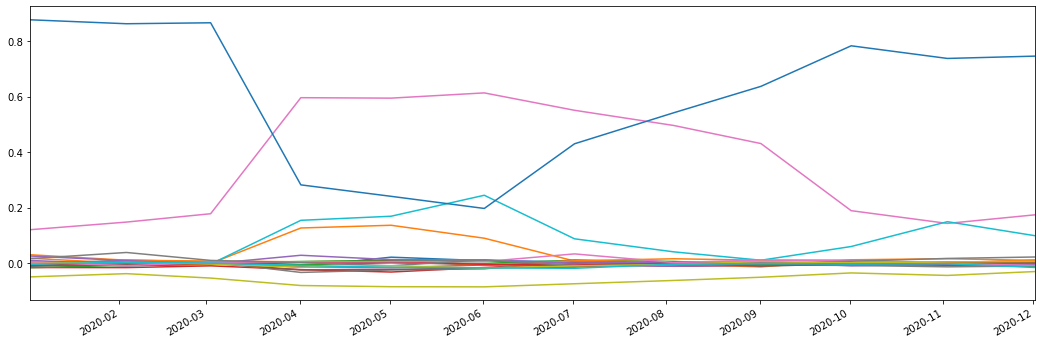
\includegraphics[width=1.15\textwidth]{bilder/MMVP-LW_allocation.png}
            \caption{MMVP-LW Target Allocation over Time}
            \label{fig:MMVP-LW_allocation_plot}
        \end{figure}
        
        % Data
        \begin{figure}[h!]
            \centering
            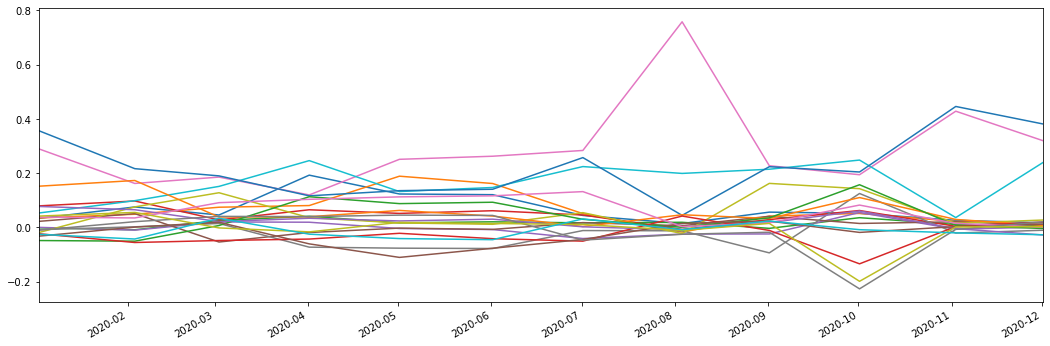
\includegraphics[width=1.15\textwidth]{bilder/MMVP-DN-K4_allocation.png}
            \caption{MMVP-DN-K4 Target Allocation over Time}
            \label{fig:MMVP-DN-K4_allocation_plot}
        \end{figure}
        
        % Data
        \begin{figure}[h!]
            \centering
            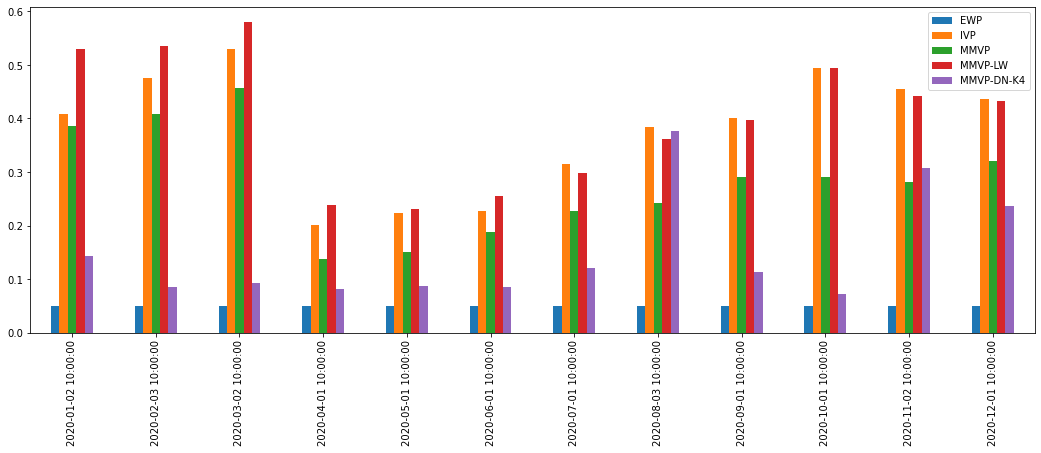
\includegraphics[width=1.15\textwidth]{bilder/nHHI_EWP_IVP_MMVP_MMVP-LW_MMVP-DN-K4.png}
            \caption{nHHIn over Time}
            \label{fig:nHHI_EWP_IVP_MMVP_MMVP-LW_MMVP-DN-K4}
        \end{figure}
        
        % Data
        \begin{figure}[h!]
            \centering
            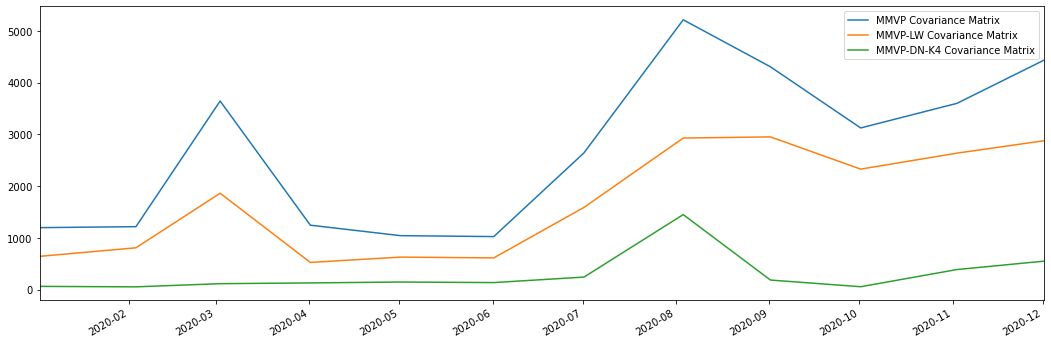
\includegraphics[width=1.15\textwidth]{bilder/Covariance_matrix_cond_comparison.png}
            \caption{Input Covariance Matrix' Condition Number over Time}
            \label{fig:Covariance_matrix_cond_comparison}
        \end{figure}
        
        % Data
        \begin{figure}[h!]
		    \centering
		    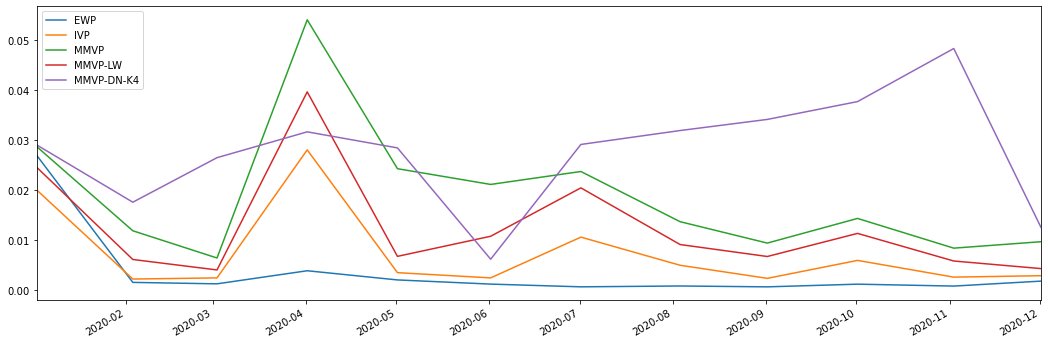
\includegraphics[width=1.15\textwidth]{bilder/Turnover_over_time_EWP_IVP_MMVP_MMVP-LW_MMVP-DN-K4.png}
		    \caption{Turnover of EWP, IVP, MMVP, MMVP-LW and MMVP-DN-K4 over The Backtesting Period}
		    \label{fig:Turnover_over_time_EWP_IVP_MMVP_MMVP-LW_MMVP-DN-K4}
		\end{figure} \todo[inline]{Missing this chart in HRP}
    
%\subsection{Equal Weight and Inverse Variance Allocation}
%    \textit{The 2 methods in this section are naive approaches to portfolio optimisation. Nevertheless, I think they are a good benchmark to compare the rest of methods. Moreover, we can also use them to see if portfolio optimisation is at all useful.}
%    
%    References: \cite{equalweight}, \cite{berndscherer}
%    
%    \subsubsection{Practical Implementation}
%        \textit{Analyse results comparing the method to Markowitz's method.}
    
\subsection{Hierarchical Risk Parity}
    %\textit{This subsection, together with subsection \ref{nassetssec}, is the biggest part of the thesis. I will describe the method in a more mathematical way, as we already discussed. Moreover, I will discuss the differences between this method and the original method of Markowitz, the model assumptions and also its limitations.}
    
    In this section, we present an alternative risk-based portfolio allocation model that lies between Markowitz minimum volatility portfolio and the inverse variance portfolio.
    
    In \cite{lopezmain}, López de Prado argues that the correlation matrix of asset returns is a linear algebra object that measures the cosines of the angles between any two vectors in the vector space formed by the returns time-series
    
    \begin{definition}
        Let $x, y \in \mathbb{R}^N \setminus \{ 0 \}$, then the \textbf{cosine of the angle between $x$ and $y$} is defined as
        \begin{align*}
            \cos \theta(x, y) := \frac{\langle x, y \rangle}{ \| x \|_2 \| y \|_2}
        \end{align*}
        where $\langle \cdot, \cdot, \rangle$ is the Euclidean scalar product in $\mathbb{R}^N$.
        
        Two vectors are consider "close" when the angle $\theta(x, y)$ is "small", i.e. when $\cos \theta(x, y)$ is "close" to $1$.
    \end{definition}
    
    \begin{theorem}
        Let $R \in \mathbb{R}^{N \times T}$ be a matrix that contains the past $T \in \mathbb{N}$ periods returns of $N \in \mathbb{N}$ assets and let $P := [\rho_{i,j}]_{i,j = 1, \dots, N} \in \mathbb{R}^{N \times N}$ be the corresponding sample correlation matrix. Then $\rho_{i,j}$ is equal to the cosine of the angle between the row vectors $\tilde{r_i}, \tilde{r_j} \in \mathbb{R}^T$ containing the centred $T$ past period returns of asset $i,j \in \{ 1, \dots, N \}$ up to some constant factor.
    \end{theorem}
    
    \begin{proof}
        Let $r_i, r_j \in \mathbb{R}^T$ be the vectors containing the past $T$ periods returns of assets $i,j \in \{ 1, \dots, N \}$, then the corresponding centred vectors of past returns are given by
        \begin{align*}
            \tilde{r_k} := \begin{bmatrix}
                r_{k,1} - \mu_k \\
                \vdots \\
                r_{k,T} - \mu_k
            \end{bmatrix} \quad \text{where} \quad \mu_k := \frac{1}{T} \sum_{t=1}^T r_{k,t} \quad \text{for} \quad k = i,j
        \end{align*}
        See definition \ref{definition:CovarianceMatrix}.
        
        Using $\tilde{r_i}, \tilde{r_j}$, we can compute the unbiased sample variance $\sigma_i^2, \sigma_j^2$ of assets $i,j$ and their unbiased covariance $\sigma_{i,j}$.
        \begin{align*}
            \sigma_k &:= \frac{1}{T-1} \sum_{t=1}^T (r_{k,t} - \mu_k)^2 = \frac{1}{T-1} (\tilde{r_k}^T \tilde{r_k}) \qquad \qquad \text{for} \quad k = i,j\\
            \sigma_{i,j} &:= \frac{1}{T-1} \sum_{t=1}^T (r_{i,t} - \mu_i) (r_{j,t} - \mu_j) = \frac{1}{T-1} (\tilde{r}_i^T \tilde{r}_j)
        \end{align*}
        Knowing the sample variances and sample covariance, we can compute the sample correlation $\rho_{i,j}$ between the past $T$ returns of asset $i$ and asset $j$.
        \begin{align*}
            \rho_{i,j} := \frac{\sigma_{i,j}}{\sqrt{\sigma_i^2} \sqrt{\sigma_j^2}} = \frac{\frac{1}{T-1} (\tilde{r}_i^T \tilde{r}_j)}{\sqrt{\frac{1}{T-1} (\tilde{r_i}^T \tilde{r_i})} \sqrt{\frac{1}{T-1} (\tilde{r_j}^T \tilde{r_j})}} = \frac{1}{\sqrt{T}} \frac{\langle \tilde{r}_i, \tilde{r}_j \rangle}{\| r_i \|_2 \| r_j \|_2} = \frac{1}{\sqrt{T}} \cos \theta(\tilde{r}_i, \tilde{r}_j)
        \end{align*}
    \end{proof}
    
    When computing Markowitz minimum volatility portfolios with algorithm \ref{algorithm:MMVP}, assets are considered as being all equal, and only their correlations/covariances are used to decide what weight an asset gets in the resulting portfolio. That means, that there is no hierarchy. This has as consequence that, in algorithmic terms, all assets are potential substitutes of each other if their covariances are low enough. López de Prado describes this by modelling the vector spaced formed by the returns series as a fully connected graph that contains a node for each asset and where each edge represents the correlation between the two assets whose nodes it connects. In economic terms, this means that, using our practical implementation framework as example, the agricultural commodities ETP is directly competing for portfolio allocation with the technology sector ETP, even though the asset classes that they represent and assets contained in each of the ETPs are very different: the returns of companies in the technology sector are driven by very different factors than the returns of wheat for example. Introducing hierarchy to the optimisation process could help to get rid of this problem, and also help to approach the asset allocation problem from a more sensible economic perspective, by allowing allocating wealth from a top-down approach. A top down approach is used by many asset managers, and consists in allocating portions of the portfolio to each asset class first, then within each asset class to each region, within each region to each industry, etc. In our practical implementation framework, this would imply that similar assets would compete for allocation between each other, and not with non-similar assets. López de Prado main contribution is to define the Hierarchical Risk Parity (HRP) model that clusters similar assets into groups recursively to later allocate portions of the portfolio to each of the groups starting from the biggest, and then further dividing allocation among the smaller groups contained in the bigger ones (top-down approach).
    
    The HRP model is divided into 3 parts:
    \begin{enumerate}
        \item Tree Clustering.
        \item Quasi-Diagonalisation.
        \item Recursive Bisection.
    \end{enumerate}
    
    The first two deal with the problem of classifying assets into clusters that contain similar assets, and the third part deals with the allocation problem among and between the asset clusters built in the first 2 steps.
    
    \subsubsection{Tree Clustering and Quasi-Diagonalisation}
        In the first step of the HRP algorithm, a hierarchical structure in form of a tree is built using the covariance matrix as input to define a metric space, in which the distance between assets can be defined as a measure of similarity. In the second step the covariance matrix is reordered so that the largest covariances lie on the diagonal.
        
        \begin{definition}[\cite{lopezmain}]\label{definition:distancematrix}
            Let $R \in \mathbb{R}^{N \times T}$ be a matrix that contains the past $T \in \mathbb{N}$ periods returns of $N \in \mathbb{N}$ assets and let $P := [\rho_{i,j}]_{i,j = 1, \dots, N} \in \mathbb{R}^{N \times N}$ be the corresponding sample correlation matrix. We define the \textbf{matrix of distances between each pair of assets $D \in \mathbb{R}^{N \times N}$} and the \textbf{matrix of distances between each asset and the rest of assets $\tilde{D} \in \mathbb{R}^{N \times N}$} as
            \begin{align*}
                D &:= [d_{i,j}]_{i,j=1, \dots, N} \quad \text{where} \quad d_{i,j} := \sqrt{\frac{1}{2} \left( 1 - \rho_{i,j} \right)} &\quad \text{for} \quad i,j = 1, \dots, N \\
                \tilde{D} &:=  [\tilde{d}_{i,j}]_{i,j=1, \dots, N} \quad \text{where} \quad \tilde{d}_{i,j} := \sqrt{\sum_{n=1}^N \left( d_{n,i} - d_{n,j} \right)} &\quad \text{for} \quad i,j = 1, \dots, N
            \end{align*}
        \end{definition}
        
        \begin{theorem}
            Let $D := [d_{i,j}]_{i,j=1, \dots, N}$ be a matrix of distances between each pair of assets as in definition \ref{definition:distancematrix}. Then $d: \mathbb{R}^T \times \mathbb{R}^T \rightarrow [0,1], d[r_i, r_j] := d_{i,j}$ is a metric for $r_i, r_j$ vectors of $T$ past returns of assets $i,j \in \{ 1, \dots, N \}$.
        \end{theorem}
        
        López de Prado provides a simple proof for this theorem in \cite{lopezmain} by showing that the defined metric is linear multiple of the Euclidean distance between the z-standardised vectors of returns, i.e. after subtracting their mean and dividing by their standard deviation.\todo[inline]{add proof?}
        
        Once we have the matrix of distances between each asset and the rest of assets $\tilde{D}$, we can start clustering similar assets into groups. This is done iteratively using the linkage criterion. Initially there are $N$ clusters $u[i] := \{ i \}$ containing only one asset (asset $i$) for $i=1, \dots, N$, and the matrix $\tilde{D}$ can be interpreted as the table that contains the distances between each pair of clusters.
        \begin{align*}
            \tilde{D} := \begin{blockarray}{ccccc}
                            u[1] & u[2] & \dots & u[N] \\
                                \begin{block}{[cccc]c}
                                  \tilde{d}_{1,1} & \tilde{d}_{1,2} & \dots & \tilde{d}_{1,N} & u[1] \\
                                  \tilde{d}_{2,1} & \tilde{d}_{2,2} & \dots & \tilde{d}_{2,N} & u[2] \\
                                  \vdots & \vdots & \ddots & \vdots & \vdots \\
                                  \tilde{d}_{N,1} & \tilde{d}_{N,2} & \dots & \tilde{d}_{N,N} & u[N] \\
                                \end{block}
                            \end{blockarray}
        \end{align*}
        
        \begin{algorithm}[H]
            \SetAlgoLined
            \SetKwInOut{Input}{Input}\SetKwInOut{Output}{Output}
            \Input{Matrix of distances between each asset and the rest of assets $\tilde{D} \in \mathbb{R}^{N \times N}$}
            \Output{Set $U$ containing the nested clusters of assets}
            
            Initialise $U := \{ \{1 \}, \dots, \{ N \} \}$\;
            %Initialise linkage matrix $Y \in \mathbb{R}^{(N-1) \times 4}$\;
            \For{$n=1$ to $N-1$}
                {
                Set $u^* := \{ v^*, w^* \} = \arg\min_{v, w \in U, v \neq w} \tilde{d}_{v,w}$ \tcp*{\footnotesize{Find the 2 nearest clusters.}}
                Set $U = (U \setminus \{ v^*, w^* \}) \cup \{ u^* \}$\;
                Delete the $v^*, w^*$ rows and $v^*, w^*$ columns from $\tilde{D}$\;
                Add row and column $\tilde{d}_{u^*} := \left[ \min_{u \in u^*} \{ \tilde{d}_{v,u} \} \right]_{v \in U}$ to $\tilde{D}$, where $\tilde{d}_{u^*,u^*} := 0$
                }
            
            \caption{Tree Clustering Algorithm}
        \end{algorithm}
        ~\
        
        López de Prado provides a short example of this algorithm in \cite{lopezmain}.
        
        \begin{example}[\cite{lopezmain}]\label{example:treeclustering}
            For better understanding, we denote each of the elements in the algorithm that we mention in the example with a subscript indicating the step in the for-loop to which they correspond.
            
            Let the initial matrix of distances between each asset and the rest of assets $\tilde{D}_0 \in \mathbb{R}^{3 \times 3}$ be given by
            \begin{align*}
                \tilde{D}_0 := \begin{blockarray}{cccc}
                                    u[1] & u[2] & u[3] \\
                                        \begin{block}{[ccc]c}
                                          0 & 0.5659 & 0.9747 & u[1] \\
                                          0.5659 & 0 & 1.1225 & u[2] \\
                                          0.9747 & 1.1225 & 0 & u[3] \\
                                        \end{block}
                                \end{blockarray}
            \end{align*}
            where the initial clusters $u[i] := \{ i \}$ only contain one asset for $i=1, \dots, 4$. Moreover, initialise the set $U_0 := \{ u[i] \; : \; i=1, \dots, N \}$. Because we only have three clusters (assets) initially, we only need to run the steps inside the for-loop twice.
            
            \textbf{First Iteration.} From the entries of the matrix $\tilde{D}_0$, we can read that the nearest clusters are $u[1]$ and $u[2]$. We proceed to create a new cluster $u_1^* := \{ u[1], u[2] \}$ that contains these two nearest clusters and to update the set of clusters to $U_1 := \{ u[3], u_1^* \} = \{ u[3], \{ u[1], u[2] \} \}$.
            
            Now, we can update the matrix $\tilde{D}_0$. First, we compute the column $\tilde{d}_{u_1^*}$.
            \begin{align*}
                \tilde{d}_{u_1^*} := \begin{bmatrix}
                    0.9747 \\
                    0
                \end{bmatrix}
            \end{align*}
            
            We denote the updated matrix $\tilde{D}_0$ as $\tilde{D}_1$.
            \begin{align*}
                \tilde{D}_1 := \begin{blockarray}{ccc}
                                    u[3] & u_1^* \\
                                        \begin{block}{[cc]c}
                                          0 & 0.9747 & u[3] \\
                                          0.9747  & 0 & u_1^* \\
                                        \end{block}
                                \end{blockarray}
            \end{align*}
            
            \textbf{Second Iteration.} Because we only have 2 clusters left, these are also the closest clusters. We process to create a new cluster $u_2^* := \{ u[3], u_1^* \}$ that contains these two nearest clusters and to update the set of clusters to $U_2 := \{ u_2^* \} := \{ \{ u[3], \{ u[1], u[2] \} \} \}$.
            
            Now, we can update the matrix $\tilde{D}_1$. First, we compute the column $\tilde{d}_{u_2^*}$.
            Now, we can update the matrix $\tilde{D}_0$. First, we compute the column $\tilde{d}_{u_1^*}$.
            \begin{align*}
                \tilde{d}_{u_2^*} := \begin{bmatrix}
                    0
                \end{bmatrix}
            \end{align*}
            
            We denote the updated matrix $\tilde{D}_1$ as $\tilde{D}_2$.
            \begin{align*}
                \tilde{D}_2 := \begin{blockarray}{cc}
                                    u_2^* \\
                                        \begin{block}{[c]c}
                                          0 & u_2^* \\
                                        \end{block}
                                \end{blockarray}
            \end{align*}
            
            The algorithm then terminates and returns the set of clusters $U_2 := \{ \{ u[3], \{ u[1], u[2] \} \} \}$.
        \end{example}
        
        After grouping the assets in clusters iteratively, the HRP algorithm uses the hierarchical structure defined by the clusters to reorganise the rows and columns of the covariance matrix, so that similar assets are placed together. To do this, rows and columns are resorted so that the rows and columns corresponding to assets that are contained in the same cluster are contiguous. This results in the covariances of asset returns pairs corresponding to the highest correlations to lie along the diagonal of the covariance matrix.
        
        \begin{example}
            Let the covariance matrix of asset returns used to compute the matrix of distances between each asset and the rest of assets $\tilde{D}_0$ given in example \ref{example:treeclustering} be defined as follows
            \begin{align*}
                \Sigma := \begin{blockarray}{cccc}
                                    u[1] & u[2] & u[3] \\
                                        \begin{block}{[ccc]c}
                                          \sigma_{1,1} & \sigma_{1,2} & \sigma_{1,3} & u[1] \\
                                          \sigma_{2,1} & \sigma_{2,2} & \sigma_{2,3} & u[2] \\
                                          \sigma_{3,1} & \sigma_{3,2} & \sigma_{3,3} & u[3] \\
                                        \end{block}
                                \end{blockarray} \in \mathbb{R}^{3 \times 3}
            \end{align*}
            
            Using the result of the tree clustering algorithm computed in example \ref{example:treeclustering}, we can compute the corresponding quasi-diagonalised covariance matrix, which is given by
            \begin{align*}
                \Sigma_{Quasi-diag} := \begin{blockarray}{cccc}
                                    u[3] & u[1] & u[2] \\
                                        \begin{block}{[ccc]c}
                                          \sigma_{3,3} & \sigma_{3,1} & \sigma_{3,2} & u[3] \\
                                          \sigma_{1,3} & \sigma_{1,1} & \sigma_{1,2} & u[1] \\
                                          \sigma_{2,3} & \sigma_{2,1} & \sigma_{2,2} & u[2] \\
                                        \end{block}
                                \end{blockarray} \in \mathbb{R}^{3 \times 3}
            \end{align*}
        \end{example}
        
    \subsubsection{Recursive Bisection}
        Once we have established a hierarchical structure of the assets by computing the set of clusters $U$ and the quasi-diagonal covariance matrix of asset returns $\Sigma_{Quasi-diag}$ as described in the previous section, we can use them to compute a target portfolio.
        
        Because the quasi-diagonalised covariance matrix is similar to a diagonal matrix, we can take advantage of the fact that the inverse-variance allocation corresponds to Markowitz minimum volatility allocation given a diagonal matrix to compute a target portfolio by defining the variance of an asset cluster as the variance of the inverse variance allocation of the portfolio containing only the assets in the cluster (bottom-up allocation approach), and by splitting allocations between adjacent clusters in inverse proportion to their aggregated variances (top-down allocation approach).
        
        \begin{algorithm}[H]\label{algorithm:hrp}
            \SetAlgoLined
            \SetKwInOut{Input}{Input}\SetKwInOut{Output}{Output}
            \Input{Set $U$ containing the nested clusters of assets and quasi-diagonal covariance matrix of asset returns $\Sigma_{Quasi-diag} \in \mathbb{R}^{N \times N}$}
            \Output{Hierarchical Risk Parity Portfolio $w \in \mathbb{R}^N$}
            
            Initialise $w_i = 1$ for all $i=1, \dots, N$\;
            Initialise $L := U$\;
            \If{$| L_i | = 1$ for all $L_i \in L$}{
                Stop\;
            }
            \Else{
            \ForEach{$L_i \in L$ such that $| L_i | > 1$}{
                    Split the cluster $L_i$ into the two sub-clusters $L_i^{(1)}, L_i^{(2)}$ that compose it\;
                    For $j=1,2$, define the variance of each sub-cluster as $\tilde{V}_i^{(j)} := \tilde{w}_j^T \Sigma_i^{(j)} \tilde{w}_j^T$, where $\Sigma_i^{(j)}$ is the covariance matrix between the assets contained in sub-cluster $L_i^{j}$, and $\tilde{w}_j^T$ is the inverse variance portfolio as in definition \ref{definition:InverseVariancePortfolio} using $\Sigma_i^{(j)}$ as input\;
                    Set $\alpha_i := 1 - \frac{\tilde{V}_i^{(1)}}{\tilde{V}_i^{(1)} + \tilde{V}_i^{(2)}}$\;
                    
                    \ForEach{asset $k$ in cluster $L_i^{(1)}$}{
                        Set $w_k = \alpha_i w_k$\;
                    }
                    
                    \ForEach{asset $k$ in cluster $L_i^{(2)}$}{
                        Set $w_k = (1 - \alpha_i) w_k$\;
                    }
                }
            Go to 3\;
            }
            
            \caption{Recursive Bisection}
        \end{algorithm}
        ~\
        
        The output of algorithm \ref{algorithm:hrp} above defines the \textbf{Hierarchical Risk Parity Portfolio}, which does not have an analytical definition as is the case for all other portfolios previously defined (EWP, IVP, MMVP, etc.).
        
        The bottom-up allocation approach can be observed in line 9 of the algorithm, where the variance of each sub-cluster is defined as the variance of the inverse allocation portfolio that contains only the assets included in the given sub-cluster.
        
        The top-down allocation approach can be observed in line 10, where the allocation to each sub-cluster is defined as the inverse variance portfolio considering a set of only two assets, in this case the two sub-clusters. This can be easily seen using the definition \ref{definition:InverseVariancePortfolio}. Let $w \in \mathbb{R}^2$ be the IVP for the set of investable assets $A := \{ L_i^{(1)}, L_i^{(2)} \}$, then $w$ is given by
        \begin{align*}
            w := \begin{bmatrix}
                w_1 \\
                w_2
            \end{bmatrix} \quad \text{where} \quad w_1 &:= \frac{\frac{1}{\tilde{V}_i^{(1)}}}{\sum_{k=1}^2 \frac{1}{\tilde{V}_i^{(k)}}} = 1 - \frac{\tilde{V}_i^{(1)}}{\tilde{V}_i^{(1)} + \tilde{V}_i^{(2)}} = \alpha_i \\
            w_2 &:= \frac{\frac{1}{\tilde{V}_i^{(2)}}}{\sum_{k=1}^2 \frac{1}{\tilde{V}_i^{(k)}}} = 1 - \frac{\tilde{V}_i^{(2)}}{\tilde{V}_i^{(1)} + \tilde{V}_i^{(2)}} = 1 - \alpha_i
        \end{align*}
        
        Finally, for the portfolio weights $0 \leq w_k \leq 1$ for all $k=1, \dots, N$ holds throughout the algorithm, because they are initialised to $1$ and only changed by a multiplication at steps 12 and 15, where $0 \leq \alpha_i \leq 1$ holds for all multiplication factors. $\sum_{k=1}^N w_k = 1$ also holds throughtout the algorithm, because the weights of higher hierarchical levels are split at each iteration, i.e. the multiplication factors at steps 12 and 15 add up to $1$.
    
    References: \cite{lopezmain}, \cite{berndscherer} \cite{stefanjansen}
    
    \subsubsection{Practical Implementation}
        \textit{Analyse results comparing the method to Markowitz's method and also to the other 3 methods above.}
        % Data
        \begin{table}[h!]
            \centering
            \begin{tabular}{crr}
             \textbf{Portfolio Optimisation Method} & \textbf{Sharpe Ratio} & \textbf{Turnover} \\
             \hline
             EWP & 0.36 & 0.003634 \\
             IVP & 1.008 & 0.007396 \\
             MMVP & -0.017 & 0.018856 \\
             MMVP-LW & 0.5 & 0.012527 \\
             MMVP-DN-K4 & -0.134 & 0.027798 \\
             HRP & 1.097 & 0.008984
            \end{tabular}
            \caption{Sharpe Ratio and Turnover Figures}
            \label{tab:all_sharpe_turnover}
        \end{table}
        
        
        % Data
        \begin{figure}[h!]
            \centering
            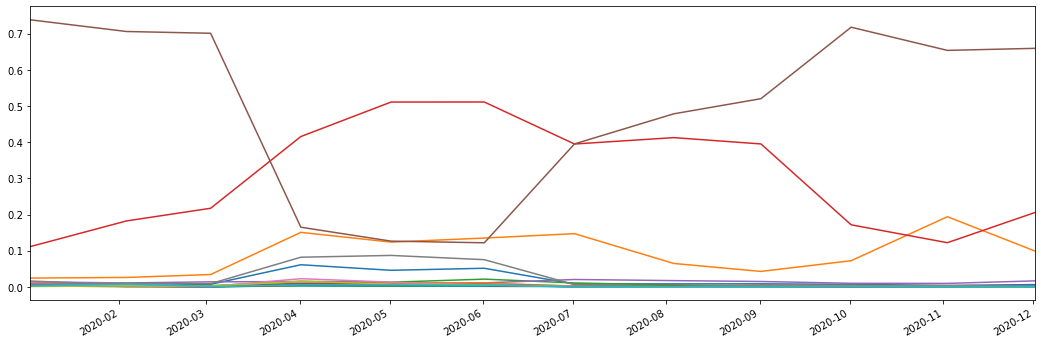
\includegraphics[width=1.15\textwidth]{bilder/HRP_allocation.png}
            \caption{HRP Target Allocation over Time}
            \label{fig:HRP_allocation_plot}
        \end{figure}
        
        % Data
        \begin{figure}[h!]
            \centering
            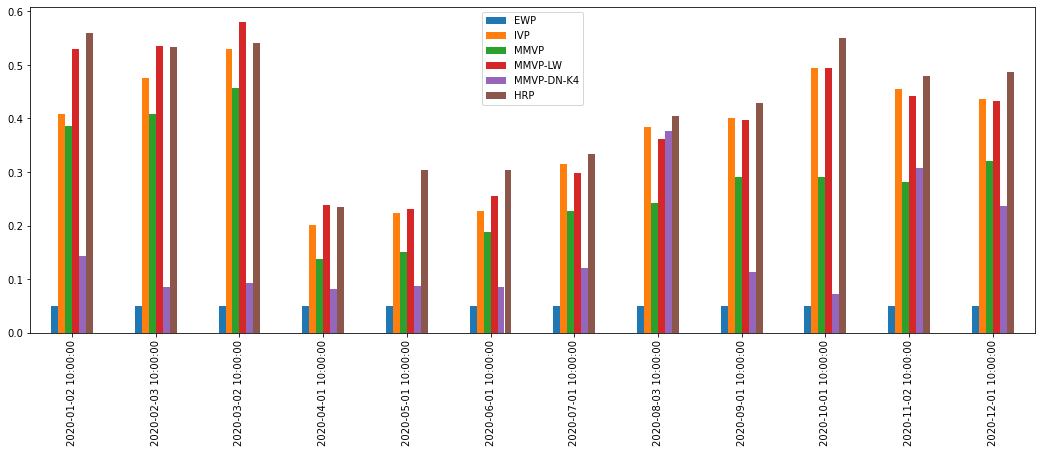
\includegraphics[width=1.15\textwidth]{bilder/nHHI_all.png}
            \caption{nHHIn over Time}
            \label{fig:nHHI_all}
        \end{figure}